\documentclass[final]{beamer}
\usetheme{GreatBritain}
\usecolortheme{Lincolnshire}
%%\usepackage[orientation=portrait,size=a1,scale=0.9,debug]{beamerposter}
%%\usepackage[orientation=portrait,size=a2,scale=0.55,debug]{beamerposter}
\usepackage[orientation=landscape,size=a0,scale=3.7,debug]{beamerposter}
\setbeamertemplate{caption}[numbered]

\usepackage{setspace}
\usepackage{color}
\usepackage{graphicx}
\usepackage{url}
\usepackage{verbatim}
\usepackage{caption}
\usepackage{subcaption}
% HEADER-BEAMER
% specifically for use in presentations

% a % sign means the rest of the line is ignored
% modify page size and spacing at end

% PREAMBLE
\usepackage{graphicx}
\usepackage{amsmath}
\usepackage{amsfonts}
\usepackage{url}

% format for environments follows
% \newenvironment{name}{starting text}{finishing text}

% matrix and determinant environments follow
\newenvironment{mat}{\left[ \begin{array}}{\end{array} \right]}
\newenvironment{deter}{\left| \begin{array}}{\end{array} \right|}

% controls the way equations are numbered
%\numberwithin{equation}{section}
% format for lists follows
% \begin{list}{label for items}{declarations} items in list \end{list}

% lista, listr, listar, listq are list environments with
% small letters, small roman numerals, arabic numerals and no item labels
\newcounter{ctr}
\newenvironment{lista}{\begin{list}{(\alph{ctr})}%
{\usecounter{ctr}
\setlength{\itemsep}{0mm} \setlength{\topsep}{-2mm}
\setlength{\leftmargin}{3em}}}{\end{list}}

\newcounter{ctr1}
\newenvironment{listr}{\begin{list}{(\roman{ctr1})}%
{\usecounter{ctr1}
\setlength{\itemsep}{0mm} \setlength{\topsep}{-2mm}
\setlength{\leftmargin}{3em}}}{\end{list}}

\newcounter{ctr2}
\newenvironment{listar}{\begin{list}{\arabic{ctr2}.}%
{\usecounter{ctr2}
\setlength{\itemsep}{0mm} \setlength{\topsep}{-2mm}
\setlength{\leftmargin}{3em}}}{\end{list}}

\newenvironment{listq}{\begin{list}{}%
{
\setlength{\itemsep}{0mm} \setlength{\topsep}{-2mm}
\setlength{\leftmargin}{3em}}}{\end{list}}

% environments for an example, examples or exercises follow

\newenvironment{exercises}{\begin{trivlist} \item[]
{\bf Exercises} \begin{enumerate}}{\end{enumerate} \end{trivlist}}


% commands for number sets follow
\newcommand{\NN}{\mathbb{N}}
\newcommand{\ZZ}{\mathbb{Z}}
\newcommand{\QQ}{\mathbb{Q}}
\newcommand{\RR}{\mathbb{R}}
\newcommand{\CC}{\mathbb{C}}
\newcommand{\LL}{\mathbb{L}}

% commands for extra mathematical symbols follow
\newcommand{\half}{\frac{1}{2}}
\newcommand{\third}{\frac{1}{3}}
\newcommand{\quarter}{\frac{1}{4}}
\newcommand{\isimp}{\Leftarrow}
\newcommand{\lsim}{\stackrel{<}{_\sim}}
\newcommand{\gsim}{\stackrel{>}{_\sim}}
\newcommand{\image}{\, {\rm im}\, }
\newcommand{\rank}{\, {\rm r}\, }
\newcommand{\domain}{\, {\rm dom}\, }
\newcommand{\adjoint}{\, {\rm adj}\, }
\newcommand{\signum}{\, {\rm sgn}\, }
\newcommand{\cosec}{\, {\rm cosec}\, }
\newcommand{\cis}{\, {\rm cis}\, }
\newcommand{\sech}{\, {\rm sech}\, }
\newcommand{\cosech}{\, {\rm cosech}\, }
\newcommand{\trace}{\, {\rm trace}\, }
\newcommand{\diag}{\, {\rm diag}\, }
\newcommand{\tri}{\, {\rm tri}\, }
\newcommand{\ud}{\, {\rm d} \kern-.015em }
\newcommand{\const}{\! {\rm const.}\; }


% the following commands need 1 or 2 arguments in { }
\newcommand{\real}[1]{{\rm Re}\left( #1 \right)}
\newcommand{\modulus}[1]{\left| \kern.05em #1 \kern.05em \right|}
\newcommand{\norm}[1]{\left\| \kern.05em #1 \kern.05em \right\|}
\newcommand{\inner}[1]{\left\langle \kern.05em #1 \kern.05em \right\rangle }
\newcommand{\recip}[1]{\frac{1}{#1}}
\newcommand{\seq}[1]{\left( #1 \right)}
\newcommand{\set}[1]{\left\{ #1 \right\} }
\newcommand{\spanof}[1]{\, {\rm span} \left\{ #1 \right\} }
\newcommand{\limit}[2]{\stackrel{\lim }{_{ #1 \to #2 }}}
\newcommand{\maxover}[1]{\stackrel{\max }{_{ #1 }}}
\newcommand{\minover}[1]{\stackrel{\min }{_{ #1 }}}
\newcommand{\dislim}[2]{\renewcommand{\arraystretch}{0.8}
\begin{array}{c}\lim \\ #1 \to #2 \end{array}}
\newcommand{\pdif}[2]{\frac{\partial #1}{\partial #2}}
\newcommand{\pddif}[3]{\frac{\partial^2 #1}{\partial #2 \partial #3}}
\newcommand{\dif}[2]{\frac{\ud #1}{\ud #2}}
\newcommand{\ildif}[2]{{\rm d} #1/{{\rm d} #2 }}
\newcommand{\ilpdif}[2]{\partial #1/{\partial #2 }}
\newcommand{\ilpddif}[3]{\partial^2 #1/{\partial #2 \partial #3}}
\newcommand{\seconddif}[2]{\frac{\ud^2 #1}{\ud #2^2}}
\newcommand{\bm}[1]{\mbox{\protect\boldmath $ #1 $}}
\newcommand{\bmzero}{\mbox{\bf 0}}
\newcommand{\pick}[2]{\renewcommand{\arraystretch}{0.6}
\left( \kern-.4em \begin{array}{c} #1 \\ #2 \end{array} \kern-.4em \right) }
\newcommand{\e}[1]{{\textrm{e}}^{#1}}
\newcommand{\cov}[1]{\, {\rm cov}\left( #1 \right) }
\newcommand{\var}[1]{\, {\rm var}\left( #1 \right) }
\newcommand{\PP}[1]{\mathbb{P}\left( #1 \right)}
\newcommand{\EE}[1]{\mathbb{E} \left( #1 \right)}


%END OF PREAMBLE




%%%%%%%%%%%% Header %%%%%%%%%%%%%


% \graphicspath{{./figures/}}

% -- Header and footer information ----------------------------------
\newcommand{\footleft}{\url{http://www.lancs.ac.uk/~daviesr3}}
\newcommand{\footright}{r.davies3@lancaster.ac.uk}
\title{Compressive Sensing for Background Subtraction}
\author{Rhian Davies (1$^{st}$ year PhD student) supervised by: Idris Eckley \ \ \ \  Lyudmila Mihaylova  \ \ \ \ Nicos Pavlidis}
\institute{STOR-i DTC  \ \ \ \ Lancaster University}
% -------------------------------------------------------------------

%Lyudmila Mihaylova, Nicos Pavlidis and Idris Eckley.

% -- Main Document --------------------------------------------------
\begin{document}
\begin{frame}{}
  \begin{columns}[t]


    % -- Column 1 ---------------------------------------------------
    \begin{column}{0.24\textwidth}

      % -- Block 1-1

\setbeamercolor{block title example}%
		{fg=black,bg=white}
		\setbeamercolor{block body example} 
		{fg=black,bg=white}
			\begin{exampleblock}{\begin{LARGE}Key message\end{LARGE}}
			When analysing videos, make every pixel count.
					\end{exampleblock}  
	\vspace{5pt}


\begin{block}{Motivation}
The amount of data being collected in the world each day is rapidly increasing. Extracting useful information from the constantly growing streams of data is difficult and analysing it efficiently is even more challenging. 

\begin{figure}[h]
  \centering
  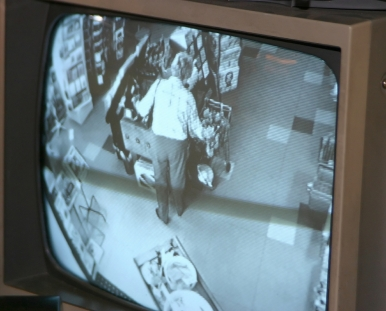
\includegraphics{bigbrother.jpg}
\end{figure}
      
A new method being employed in signal processing is compressive sensing (CS) which is a way to acquire data directly in a compressed form.
\end{block}

      \vspace{10pt}

      % -- Block 1-2
      \begin{block}{What is compressive sensing?}
Compressive sensing is a method of reducing the amount of data collected from a signal without compromising the ability to later reconstruct the signal accurately. This method will only work if the signal of interest is compressible. 
\end{block}
      \vspace{10pt}
\begin{block}{Sparsity}
A signal is compressible if most of the information in the signal is contained within a few coefficients. Most images are compressible under the wavelet basis. 

\begin{figure}[h]
  \centering
   \begin{subfigure}[b]{0.45\textwidth}
                \centering
                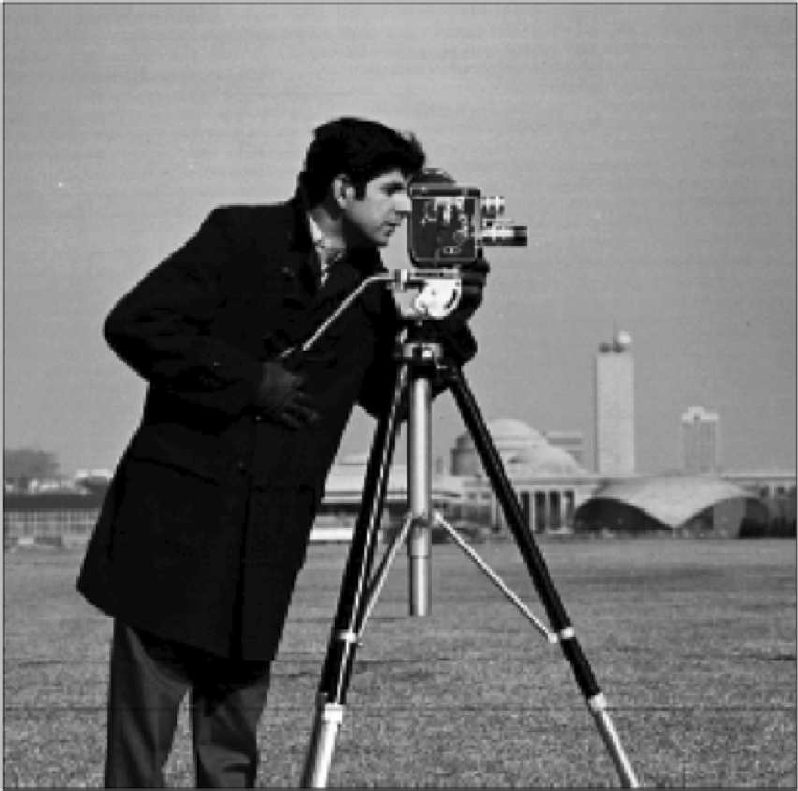
\includegraphics[width=\textwidth]{manoriginal}
                \caption{Original frame}
        \end{subfigure}
\quad
\begin{subfigure}[b]{0.45\textwidth}
                \centering
                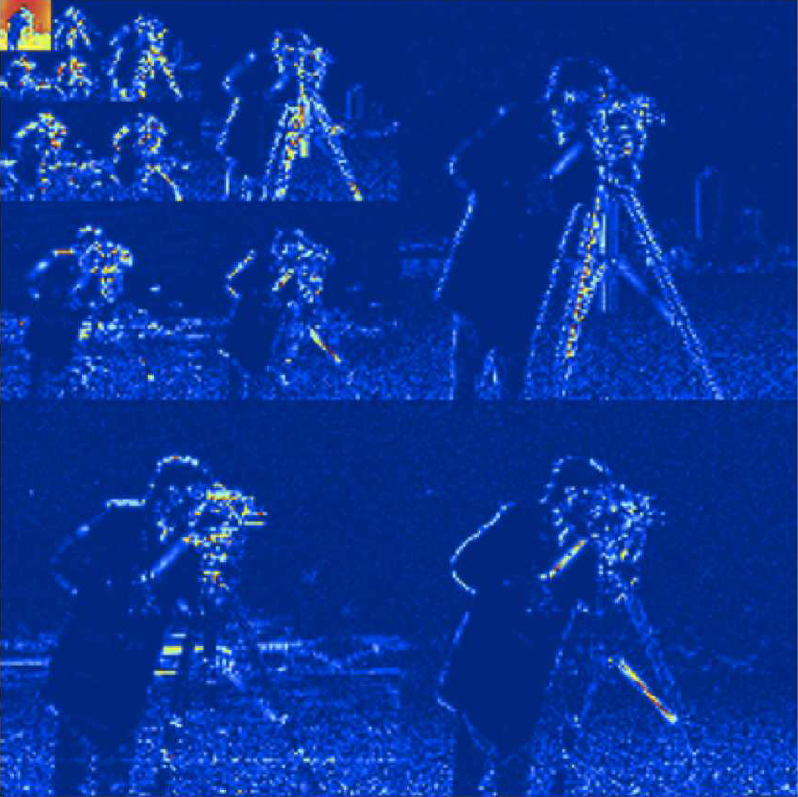
\includegraphics[width=\textwidth]{manwavelet}
                \caption{Wavelet transformation}
                \label{fig:wt}
        \end{subfigure}
  \caption{In the wavelet transformation lighter pixels refer to large transform coefficients and dark areas refer to smaller coefficients. There are only few light areas but many dark ones which implies that the image is compressible. Figure originally from Baranuik (2011).}
  \label{fig:waveletcoeff}
\end{figure}
\vspace{20pt}

\end{block}

    \end{column}%1

    % -- Column 2 ---------------------------------------------------
    \begin{column}{0.24\textwidth}

		% -- Block 2-1
		\begin{block}{CS Methodology}
Assume that the signal of interest $\pmb{x}$ is of length N.
                  \begin{itemize}
                  \item Choose $M$, the number of measurements to take of $\pmb{x}$. $(M < < N).$
                    \item Create a random measurement matrix $\pmb{\Phi}$ of size $M \times N$. This must satisfy the RIP. 
                      \item Calculate measurement $\pmb{y}$ according to equation \eqref{eq:1}.
                        \item Reconstruct $\pmb{x}$ using a recovery optimisation method.
                  \end{itemize}

\begin{figure}[h]
        \centering
        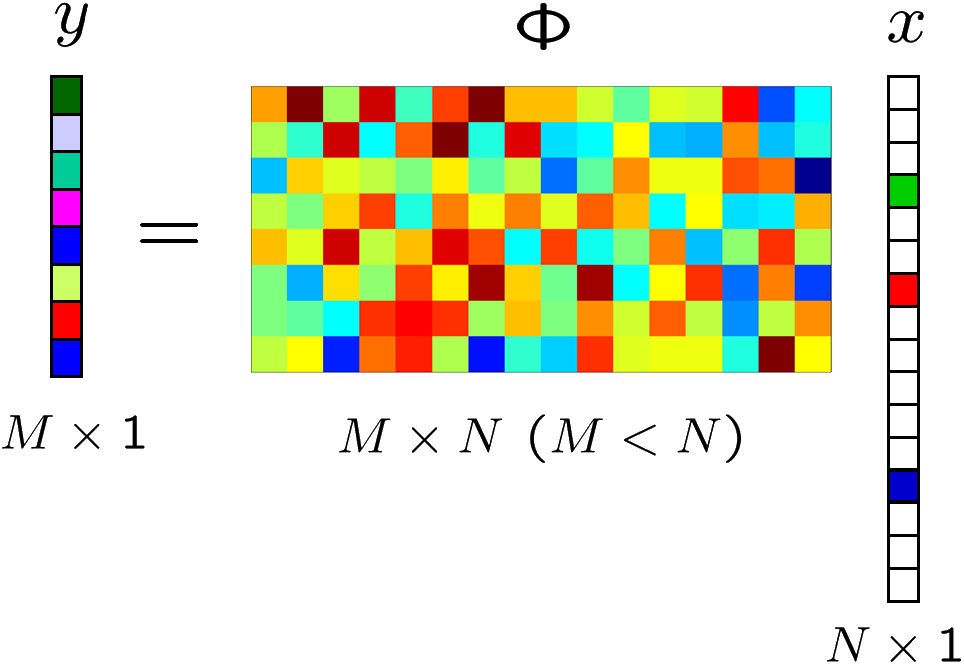
\includegraphics{csss}
        \caption{CS measurement process, courtesy of Volkan Cevher.}
      \end{figure}


\begin{equation}
  \label{eq:1}
\pmb{y} =\pmb{\Phi x}
\end{equation}


Many vectors $\pmb{\hat{x}}$ can solve equation \eqref{eq:1}, but usually $\pmb{x}$ is the only sparse solution. Therefore if $\pmb{x}$ is known in advance to be sparse, it can in theory be reconstructed exactly from $M$ measurements.
\end{block}
   \vspace{10pt}
\begin{block}{Restricted Isometry Property (RIP)}

  A matrix $\pmb{\Phi}$ satisfies the Restricted Isometry Property (RIP) of order $K$ if there exists a $\delta_K  \in (0,1)$ such that 
\begin{equation}
  \label{eq:4}
  (1 - \delta_k)||\pmb{x}||^2_2 \leq||\pmb{\Phi} \pmb{x}||^2_2 \leq (1 + \delta_k)||\pmb{x}||^2_2,
\end{equation}
for all $\pmb{x} \in \sum_K = {\pmb{x}:||\pmb{x}||_0 \leq K} $.
 
If $\pmb{\Phi}$ satisfies the RIP with order $2K$, then $\pmb{\Phi}$ preserves the distance between any pair of $K$-sparse vectors, making the recovery procedure possible.
\end{block}

      \vspace{10pt}
      
      % -- Block 2-2

      \begin{block}{Recovery of sparse transforms}
The signal $\pmb{x}$ is reconstructed by applying some recovery algorithm to $\pmb{y}$. We wish to find the $K$-sparse solution. Optimisation based on the $l_1$ norm can closely approximate compressible signals with high probability.
%
\begin{equation}
  \label{eq:3}
  \pmb{\hat{x}} = \text{arg} min_{y = \phi x} ||\pmb{x}||_1
\end{equation}
%
This $l_1$ norm minimisation problem reduces to a linear program known as basis pursuit which replaces the sparse approximation problem by a convex problem.
%An alternative to basis pursuit is a greedy algorithm called orthogonal matching pursuit (OMP). This method can be faster than basis pursuit due to its simplicity; it iteratively computes the local optimum solution in the hope that these will lead to the global optimum solution.  

\vspace{100pt}



      \end{block}

      \vspace{10pt}
      
     
      \end{column}%2
 
   % -- Column 3 ---------------------------------------------------
    \begin{column}{0.24\textwidth}

		% -- Block 3-1
		\begin{block}{Background Subtraction (BGS)}
Background subtraction is a method for segmenting the foreground and the background. Foreground is defined to be the moving objects of interest in a video sequence and the background is everything else.This information could be used to track a particular object or classify the scene as a particular event.
\vspace{20pt}
 
 \begin{figure}
                    \centering
                   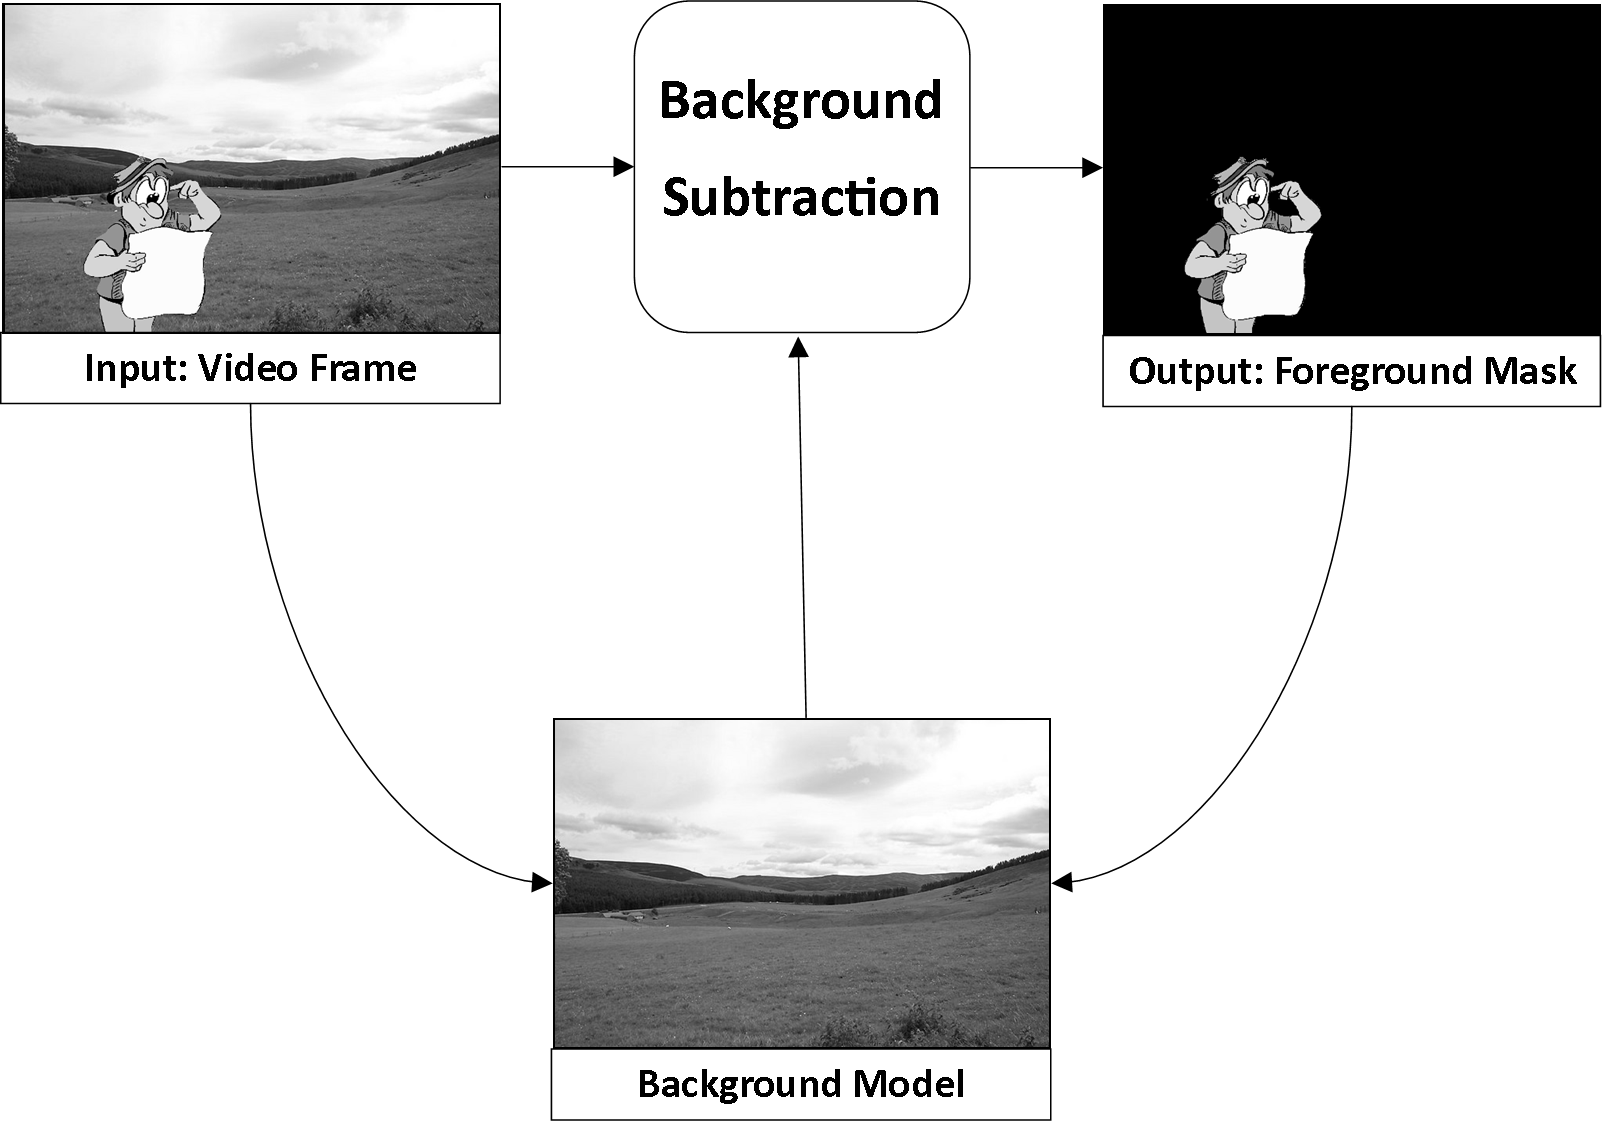
\includegraphics{backgroundsubtraction} 
\caption{The background subtraction process}
                  \end{figure}
\vspace{20pt}
A model of the background is created and then this background model is subtracted from each video frame in turn what remains is classified as the foreground. Using luminance pixel intensity, information can be stored about each video frame in matrix form. 
%\begin{figure}[h]
%  \centering
%   \begin{subfigure}[b]{0.45\textwidth}
%                \centering
%                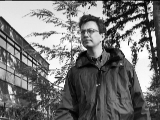
\includegraphics[width=\textwidth]{wtbw}
%                \caption{Original frame}
%        \end{subfigure}
%\quad
%\begin{subfigure}[b]{0.45\textwidth}
%                \centering
%                
\includegraphics[width=\textwidth]{wtgt}
%                \caption{Ground Truth}
%                \label{fig:wt}
%        \end{subfigure}
%  \caption{.}
%  \label{fig:waveletcoeff}
%\end{figure}

      \end{block}

      \vspace{10pt}
      
      % -- Block 3-2

%      \begin{block}{Standard techniques for background subtraction}
%Frame differencing compares the  pixel intensity of the current frame and the previous frame and thresholds.Approximate median adapts a model of the background as each frame is read. Mixture of Gaussian models pixel intensity.These techniques have been studied in depth but don't work very well when dealing with occlusions, repetitive background motion and shadows, also termed ghosts.
%\end{block}

      \vspace{10pt}
      
      % -- Block 3-34 
      \begin{block}{Compressive sensing with BGS}
My current interests involve incorporating compressive sensing with standard BGS methods as follows.
\vspace{10pt}
\begin{enumerate}
\item Create a random Gaussian measurement matrix $\pmb{\Phi}$.
\item Preprocess, read and compress background frame $\pmb{y_b}$.
\item Preprocess, read and compress next frame $\pmb{y_c}$.
\item Pixel $i$ is classed as foreground if $|y_c(i) - y_b(i)|< \tau$. 
\item Update background model $\pmb{y_b} = \pmb{y_c}$
\item Repeat from step 3.
\end{enumerate}
\vspace{10pt}
$\tau$ is a background subtraction threshold to be chosen.

\vspace{10pt}

 In reality each video frame is compressed row by row as instead of a the whole frame in one go in order to preserve the shape of the image. 


\vspace{100pt}
      \end{block}

      \end{column}%3
    
   
    % -- Column 4 ---------------------------------------------------
    
    \begin{column}{0.24\textwidth}

		% -- Block 4-1
      \begin{block}{Current Experimentation}
I am currently attempting to apply this theory on a traffic video. This video exhibits many difficulties such as shadows, occlusions and high frequency repetitive background motion. 
        \begin{figure}
          \centering
          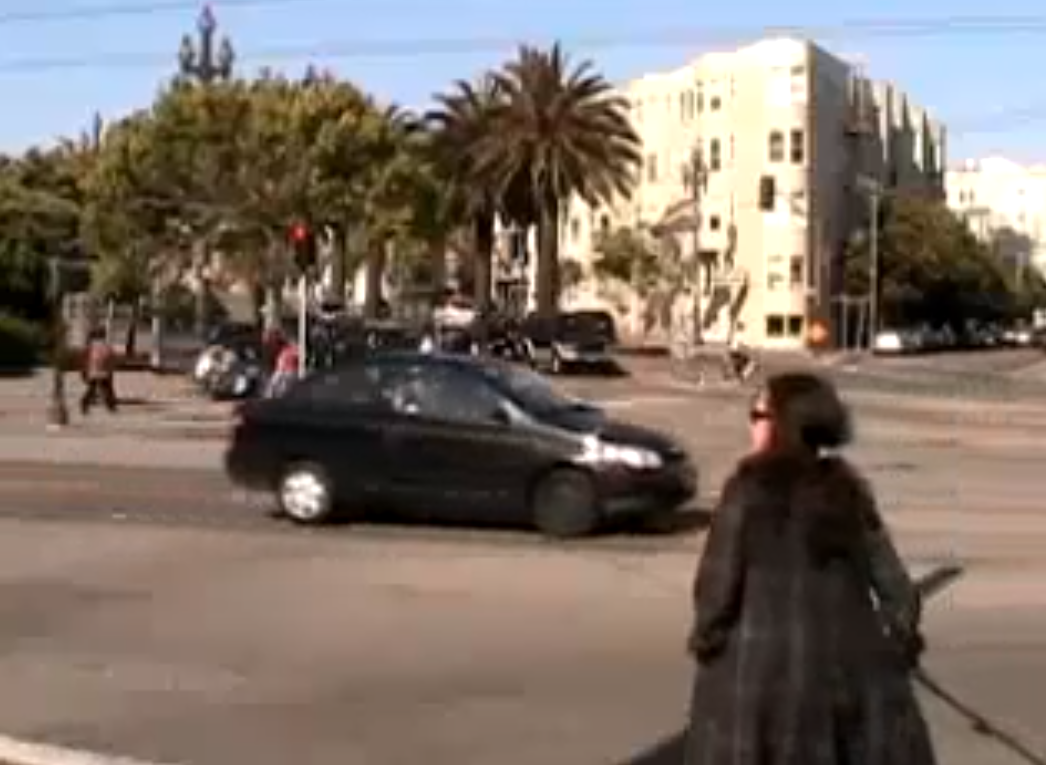
\includegraphics[width=14cm]{trafficvideo}
\caption{Sanfran test video courtesy of Seth Benton}
        \end{figure}
The aim of this experiment is to understand how different types of recovery optimisation algorithms compare against the standard basis pursuit method in terms of quality of reconstruction and computational time.

      \end{block}

      \vspace{10pt}
      
      % -- Block 4-2
      \begin{block}{Areas to explore}
        \begin{itemize}
        \item How to select a good $\Phi$? 
\item Rule of thumb for M
\item How do different distributions for $\Phi$ affect performance?
\item How well an would an adaptive $\Phi$ work?
\item Comparison of different reconstruction methods.
\item Applying compressive sensing to different methods of background subtraction
        \end{itemize}
      \end{block}

      \vspace{10pt}
      
      \begin{block}{Find out more}
        You can learn more about my research and keep in touch by following this link. 
        \begin{figure}
          \centering

\includegraphics{qr}          
        \end{figure}

      \end{block}

       % -- Block 4-3			
      \begin{block}{References}
				\begin{footnotesize}
				\begin{thebibliography}{10}

\bibitem[Eldar and Kutyniok, 2012]{EldarKutyniok2012}
Eldar, Y.C. and Kutyniok, G. (2012). Compressed Sensing.

\bibitem[Ling, 2011]{lingbaraniuk2011}
Mei, X. and Ling, H. (2011). Robust visual tracking and vehicle classification via sparse representation.

\bibitem[Baraniuk, 2007]{baraniuk2007}
Baraniuk, R.G. (2007). Compressive Sensing.
\end{thebibliography}

				\end{footnotesize}

\vspace{100pt}
      \end{block}

    \end{column}%4

  \end{columns}
\end{frame}
\end{document}
